\documentclass[a4paper]{report}

% \usepackage{a4wide}
\usepackage{graphicx}
\usepackage{wrapfig}
\usepackage[utf8]{inputenc}
\usepackage{blindtext}
\usepackage{amsmath}
\usepackage{amssymb}
\usepackage{amsfonts}
\usepackage{physics}
\usepackage{setspace}
\usepackage{mathrsfs}

\onehalfspacing

\newcommand{\problem}[1]{$\vb*{\mathsection}$ \textbf{Problema #1.}}
\newcommand{\letter}[1]{\vspace*{3mm}\textbf{(#1)} \hspace{1mm} }
\newcommand{\levicivita}[1]{\epsilon_{#1}}

\usepackage{accents}
\newcommand*{\dt}[1]{%
  \accentset{\mbox{\large\bfseries .}}{#1}}
\newcommand*{\ddt}[1]{%
  \accentset{\mbox{\large\bfseries .\hspace{-0.25ex}.}}{#1}}
\newcommand*{\dddt}[1]{%
  \accentset{\mbox{\large\bfseries .\hspace{-0.25ex}.\hspace{-.20ex}}}{#1}}
\newcommand*{\dnt}[2][4]{\dt{#2}^{\tiny(#1)}}


\newcommand{\listnumber}[1]{
  \begin{center}
    \Large
    \textbf{FIS 108 Eletrodinâmica Clássica I - Lista #1} \\
    \large
    Alex Enrique Crispim
    \normalsize
  \end{center}
}


\begin{document}
\listnumber{1}

\problem{1} \textit{Use Gauss's theorem (and (1.21) if necessary) to prove the following:}

\letter{a} \textit{Any excess charge placed on a conductor must lie on its surface. (A conductor, by definition, contains charges capable of moving freely under the action of applied electric fields.)}

Comecemos provando o Teorema de Earnshaw para argumentar que o campo elétrico no interior de um condutor deve ser nulo.

Suponha que tenha-se uma carga em uma região onde existe um campo elétrico $\vb{E} = -\grad{\Phi}$. Vamos supor que exista um ponto $P$, que não esteja na fronteira do espaço onde tem-se o campo elétrico, tal que $\Phi$ assuma um valor mínimo. Então, ao se afastar de $P$ tem-se um aumento no potencial, para qualquer direção. Podemos escrever esse fato como
\begin{equation*}
  \pdv{\Phi}{\vb{n}^\prime} = \grad{\Phi} \vdot \vu{n}^\prime > 0
  \quad \forall \vb{n}^\prime .
\end{equation*}
Tomando uma superfície fechada $S$ próxima do ponto $P$, englobando o mesmo, temos que
\begin{equation*}
  \oint_S \pdv{\Phi}{\vb{n}^\prime} \dd{a} > 0.
\end{equation*}
Por outro lado, a lei de Gauss nos fornece
\begin{equation*}
  \oint_S \pdv{\Phi}{\vb{n}^\prime} \dd{a} = \int_V \laplacian{\Phi} \dd[3]{x} = 0
\end{equation*}
contradizendo o resultado anterior. Analogamente, temos para o caso onde $P$ é um máximo do potencial.

Como consequência, temos que \textit{o potencial eletrostático só pode assumir um valor mínimo ou máximo no bordo da região onde tem-se um campo elétrico}.

Do teorema anterior, vê-se que uma carga elétrica, $q$, não pode estar em equilíbrio em uma região onde há campo elétrico, pois sua energia potencial $q\Phi$ não apresenta um mínimo, senão na borda do espaço. Assim, nenhuma configuração de cargas pode ser estável apenas por interações eletrostáticas.

Do resultado acima, se tivermos cargas no interior de um condutor, haverá um campo elétrico resultante (o que se pode ver facilmente pela lei de Gauss), levando a um potencial eletrostático, consequentemente. Como tal configuração de cargas não é estável, as mesmas tendem a ir para o bordo do espaço em questão, isto é, para a superfície do material. É claro que o bordo deve representar um mínimo do potencial, neste caso, pois se fosse um máximo, as cargas não poderiam ir para tal região, caindo no problema anterior.

Segue, portanto, que o campo elétrico no interior de um condutor deve se anular, no caso estacionário.

Um outro modo de ver este problema envolve um argumento diferente: no caso estacionário não podem haver correntes no interior do condutor, pois o movimento de correntes leva a dissipação de energia, portanto, não pode existir sem um agente externo realizando trabalho. Com isso, $\vb{E}^{(int)} = 0$.

Para mostrar que as cargas devem se distribuir na superfície do condutor, usamos a ideia desenvolvida pode Lorentz (1902) de que os campos macroscópicos podem ser obtidas tomando-se a média para os campos microscópicos. Seja $\vb{e}$ o campo elétrico microscópico, temos
\begin{equation*}
  0 = \div{\vb{E}^{(int)}} = \div{\ev{\vb{e}}} = \ev{\rho} / \epsilon_0 \Leftrightarrow \ev{\rho} = 0,
\end{equation*}
com $\rho$ sendo a densidade miscroscópica de cargas. Para anular a densidade de carga no interior, as cargas devem estar distribuidar na superfície do condutor.

\letter{b}
\textit{A clossed, hollow condutor shields its interior from fields due to charges outside, but does not shield its exterior from the fields due to charges placed inside it.}

No interior do condutor, quando não existem cargas, a Lei de Gauss fornece
\begin{equation*}
  \oint_S \vb{E} \vdot \dd{\vb{a}} = 0,
\end{equation*}
para toda superfície $S$ fechada no interior do condutor. Logo, o campo elétrico no interior deve se anular;
\begin{equation*}
  \vb{E} = 0 \quad \text{(inteior).}
\end{equation*}

Por outro lado, se existe uma carga total $q$ no interior do condutor, para uma superfície $S$ externa ao condutor, englobando o mesmo, é fácil ver que
\begin{equation*}
  \oint_S \vb{E}\vdot \dd{\vb{a}} \neq 0,
\end{equation*}
seja qual for $S$. Como existe sempre um fluxo do campo sobre a superfície, o mesmo é não nulo. Está mostrado o resultado.

\letter{c}
\textit{The electric field at the surface of a conductor is normal to the surface and has a magnitude $\sigma/\epsilon_0$, where $\sigma$ is the charge density per unit area on the surface.}

Vamos considerar a direção $z$ como sendo normal a um ponto arbitrário da superfície do condutor e olhar para o entorno desse. Lembrando que $\curl{\vb{E}} = 0$, temos o seguinte:

Podemos utilizar que
\begin{equation*}
  \oint \vb{E} \vdot \dd{\vb{l}} = 0
\end{equation*}
para deduzir uma condição de contorno para o campo elétrico ao atravessar a interface (superfície do condutor) que separa o meio interno do meio externo. Considere a figura abaixo:

\begin{figure}[h]
  \center
  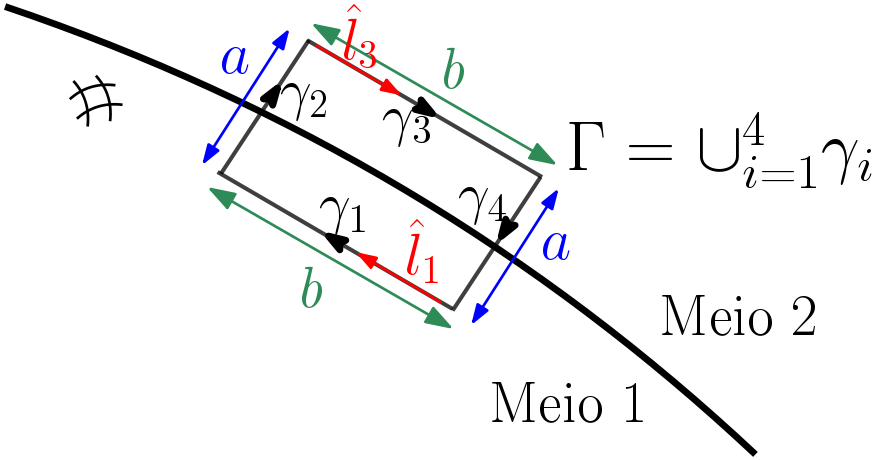
\includegraphics[scale = .27]{./imgs/matching_conditions.png}
  \caption{Diagrama de uma região infinitesimal de uma superfície de separação entre dois meios (meios 1 e 2, da figura). $\Gamma$ é um caminho retangular fechado que contém partes em ambos os meios. $a$ e $b$ são as medidas dos lados do caminho. O caminho $\Gamma$ é composto pela união dos caminhos $\gamma_j$ (j = 1,...,4), que descrevem cada lado. $\vu{l}_i$ ($i$ = 1,3) denotam os versores diretores das curvas $\gamma_i$.}
\end{figure}

Podemos escrever
\begin{equation*}
  0 = \oint \vb{E} \vdot \dd{\vb{l}} = \int_{\gamma_1} \vb{E} \vdot \dd{\vb{l}} + \int_{\gamma_2} \vb{E} \vdot \dd{\vb{l}} + \int_{\gamma_3} \vb{E} \vdot \dd{\vb{l}} + \int_{\gamma_4} \vb{E} \vdot \dd{\vb{l}}.
\end{equation*}
No limite $a \to 0$, as os caminhos $\gamma_{2,4}$ passam a não contribuir para a integral de modo que
\begin{equation*}
  \int_{\gamma_1} \vb{E} \vdot \dd{\vb{l}} + \int_{\gamma_3} \vb{E} \vdot \dd{\vb{l}} \sim 0, \quad \text{quando } a \to 0.
\end{equation*}
Considerando os versores diretores das curvas $\gamma_{1,3}$, $\vu{l}_{1,3}$, da figura, podemos calcular a integral acima sob a hipótese de que o comprimento $b$ seja muito pequeno de tal forma que o campo seja aproximadamente uniforme. Com isso,
\begin{equation*}
  \int_{\gamma_i} \vb{E}_i \vdot \dd{\vb{l}} = b \vb{E} \vdot \vu{l}_i,
\end{equation*}
Onde $\vb{E}_i$ denota o campo elétrico no meio ``$i$''.
Observando que $\vu{l}_1 = - \vu{l}_3$, podemos escrever a soma das integrais anteriores como
\begin{equation*}
  (\vb{E}_1 - \vb{E}_3) \vdot \vu{l}_1 = 0,
\end{equation*}
onde eliminamos o fator $b$, irrelevante. Notando que $\vb{E}_i \vdot \vb{l}_i$ é o campo tangencial, podemos finalmente entender a condição de contorno acima como: ``\textit{a componente tangencial do campo elétrico é constante através da interface que separa dois meios}''.

Para o caso específico de um condutor, como o campo interno é nulo, segue que a componente tangencial do campo elétrico deve se anular. Assim, o campo é normal à superfície do condutor (Figura 2 abaixo). Um outro fato importante que segue é que a superfície de um condutor é uma equipotencial. Isso segue da expressão $\vb{E} = - \grad{\Phi}$.

\begin{figure}[h]
  \center
  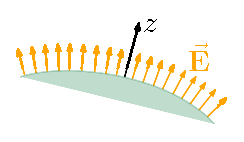
\includegraphics[scale = 1.1]{./imgs/surf.eps}
  \caption{Campo elétrico nas imediações de um condutor. O campo é normal à superfície; as linhas de campo emergem ou terminam na superfície do condutor.}
\end{figure}

Com as informações obtidas, podemos utilizar a Lei de Gauss para obter o campo elétrico na vizinhança do condutor.

Seja $\sigma$ a densidade superficial de carga no condutor, considere uma superfície $S_g$ como a representada na figura abaixo.

\begin{figure}[h]
  \center
  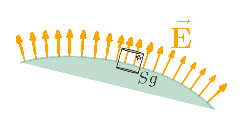
\includegraphics[scale = 1.1]{./imgs/gauss.eps}
  \caption{Superfície $S_g$ cilindrica com uma parte no interior do condutor a outra face externa ao mesmo.}
\end{figure}

Considerando o limite na qual a lateral do cilindro é muito pequena e a área das outras regiões é $A$, pela forma integral da Lei de Gauss, podemos escrever
\begin{align*}
  \frac{1}{\epsilon_0} \int_A \sigma \dd{a} = \oint_{S_g} \vb{E} \vdot \dd{\vb{a}} = \int_\text{lateral} \vb{E} \vdot \dd{\vb{a}} + \int_\text{area interna} \vb{E} \vdot \dd{\vb{a}} + \int_\text{area externa} \vb{E} \vdot \dd{\vb{a}}
\end{align*}
\begin{align*}
  \frac{\sigma A}{\epsilon_0} = 0 + 0 + \vb{E} \vdot \vu{n} A,
\end{align*}
com $\vu{n}$ sendo o vetor normal à superfície. A integral $\int_A \sigma \dd{a}$ resultou em $\sigma A$ pois a superfície $S_g$ pode ser tomada arbitrariamente pequena tal que $\sigma$ seja aproximadamente constante, localmente.
Dos resultados anteriores, $\vb{E} = E \vu{n}$, assim,
\begin{equation*}
  \vb{E} = (\sigma/\epsilon_0) \vu{n}.
\end{equation*}


\newpage
\problem{2} \statment{The Dirac delta function in three dimensions can be taken as the improper limit as $\alpha \to 0$ of the Gaussian function
\[
  D(\alpha, x, y, z) = (2\pi)^{-3/2} \alpha^{-3} \exp[-\frac{1}{2\alpha^2}(x^2 + y^2 + z^2)].
\]
Consider a general orthogonal coordinate system specified by the surfaces $u = constant$, $v = constant$, $w = constant$, with length elements $\dd{u}/U$, $\dd{v}/V$, $\dd{w}/W$ in the three perpendicular directions. Show that
\[
  \delta(\vb{x} - \vb{x}^\prime) = \delta(u - u^\prime)\delta(v - v^\prime)\delta(w - w^\prime) \cdot UVW
\]
by considering the limit of the Gaussian above. Note that as $\alpha \to 0$ only the infinitesimal length elements need be used for the distance between the points in the exponent.}

A transformação  $T \colon (x,y,z) \mapsto (u,v,w)$ entre os sistemas de coordenadas é realizada por uma aplicação invertível, bijetiva e diferenciável tal que a derivada $\mathcal{D}T$ é invertível em todo ponto.
O elemento de linha $\dd{\vb{r}}$, passa a ser
\[
  \dd{\vb{r}} = h_i \dd{q_i} \vu{e}_i = \dd{u}/U \vu{u} + \dd{v}/V \vu{v} +\dd{w}/W \vu{w}
\]
e, logo, o elemento de comprimento $\dd{s}$ passa a ser, para um sistema de coordenadas ortogonal,
\[
  (\dd{s})^2 = (\dd{u})^2/U^2 + (\dd{v})^2/V^2 + (\dd{w})^2/W^2
\]
%
% Seja $\Omega$ uma função qualquer, sua diferecial $\dd{\Omega}$ pode ser escrita como
% \begin{align*}
%   \dd{\Omega}
%     &= \pdv{\Omega}{q^i} \dd{q_i} = (\dd{\vb{r}} \vdot \grad) \Omega,
% \end{align*}
% de onde-se vemos que
% \begin{equation*}
%   \grad_i = \frac{1}{h_i} \partial_i.
% \end{equation*}
%
% A expansão em Taylor de $\Omega$, supondo que a mesma exista, pode ser escrita como
% \[
%   \Omega(\vb{r}) = \Omega(\vb{a}) + \eval{ (\vb{a} \vdot \grad) \Omega(\vb{r}) }_{\vb{a}} + \frac{1}{2!} \eval{ (\vb{a} \vdot \grad)^2 \Omega(\vb{r}) }_{\vb{a}} + ... + \frac{1}{n!} \eval{ (\vb{a} \vdot \grad)^n \Omega(\vb{r}) }_{\vb{a}} + ...
% \]
%
% Em primeira ordem, em um sistema de coordenadas curvilíneas $(q_i)$, com elementos de comprimento $h_i$, temos
% \[
%   \Omega(\vb{r}) = \Omega(\vb{a}) + \eval{ \qty(\frac{a_i}{h_i} \partial_i) \Omega(\vb{r}) }_{\vb{a}}.
% \]


Da Figura \ref{fig:gaussian-limit}, pode-se ver que, no limite $\alpha \to 0$, apenas a vizinhança do ponto \aspas{0} importa (como também mencionado no enunciado).
\begin{figure}[h]
  \center
  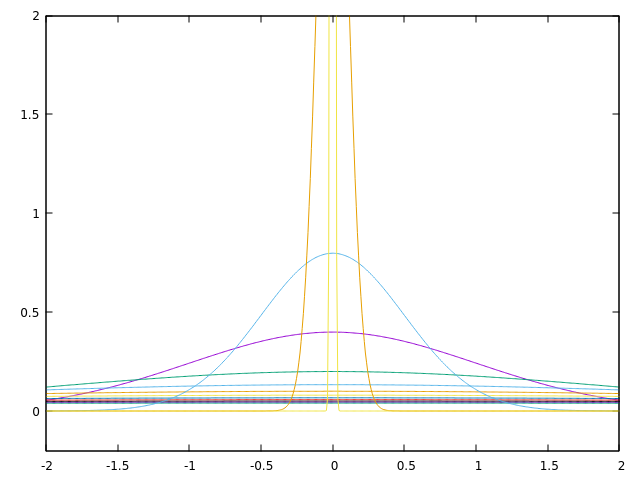
\includegraphics[scale = .4]{./imgs/gaussian_limit.png}
  \caption{Limite quando $\alpha \to 0$ da função $\frac{1}{\sqrt{2\pi} \alpha} \exp(-\frac{x^2}{2\alpha^2})$. Os picos mais elevados e estreitos representam menores valores para $\alpha$.}
  \label{fig:gaussian-limit}
\end{figure}

Com isso, no limite $\alpha \to 0$, $\Delta \vb{x}^2 = (\vb{x} - \vb{x}^\prime)^2 \sim \dd{s}^2$. Assim,
\begin{align*}
  \Delta \vb{x}^2
  &\sim (\dd{u})^2/U^2 + (\dd{v})^2/V^2 + (\dd{w})^2/W^2,
  \\
  &\sim \frac{u - u^\prime}{U^2} + \frac{v - v^\prime}{V^2} + \frac{w - w^\prime}{W^2}.
\end{align*}

A função $D(\alpha; \vb{x})$ pode ser escrita como
\begin{equation*}
  D(\alpha; \vb{x}) = (2\pi)^{-3/2} \alpha^{-3} \exp[-\frac{1}{2\alpha^2}\qty(\frac{u - u^\prime}{U^2} + \frac{v - v^\prime}{V^2} + \frac{w - w^\prime}{W^2})].
\end{equation*}

Como,
\begin{align*}
  D(\alpha; \vb{x})
  &= \qty{(2\pi)^{-1/2}\alpha^{-1} \exp[-\frac{1}{2 \alpha^2} (x-x^\prime)^2]} \qty{(2\pi)^{-1/2}\alpha^{-1} \exp[-\frac{1}{2 \alpha^2} (y-y^\prime)^2]} \times
  \\
  &\qquad  \qty{(2\pi)^{-1/2}\alpha^{-1} \exp[-\frac{1}{2 \alpha^2} (z-z^\prime)^2]}
  \\
  &\longrightarrow \delta(x - x^\prime) \delta(y - y^\prime) \delta(z - z^\prime)
\end{align*}
cada um dos termos $(2\pi)^{-1/2}\alpha^{-1} \exp[-\frac{1}{2 \alpha^2} (x_i - x_i^\prime)^2]$ tende para uma delta. Em especial,
\begin{equation*}
  (2\pi)^{-1/2}\alpha^{-1} \exp[-\frac{1}{2 Q_i^2\alpha^2} (q_i - q_i^\prime)^2] = \frac{Q_i}{\sqrt{2\pi} \alpha^\prime} \exp[-\frac{1}{{\alpha^\prime}^2}(q_i - q_i^\prime)^2] \xrightarrow[\alpha^\prime \to 0]{} Q_i \delta(q_i - q_i^\prime),
\end{equation*}
onde $\alpha^\prime = Q_i \alpha$ e $Q_i$ é o (inverso do) elemento de comprimento associado a $q_i$.

Portanto, combinando os resultados,
\begin{equation*}
  D(\alpha; \Delta\vb{x}) \xrightarrow[\alpha \to 0]{} \delta(u - u^\prime) \delta(v - v^\prime) \delta(w - w^\prime) \cdot UVW.
\end{equation*}

\vspace{5mm}
De forma mais geral, o resultado poderia ser obtido considerando-se a integral
\begin{equation*}
  \int_{\mathbb{R}^3} \delta(\vb{x}) \dd[3]{\vb{x}} = 1.
\end{equation*}
Em coordenadas curvilíneas, o elemento de volume $\dd[3]{\vb{x}}$ é transformado em
\[
  \dd[3]{\vb{x}} \to \abs{\pdv{(x, y, z)}{u, v, w}} \dd{u}\dd{v}\dd{w} = \frac{\dd{u}\dd{v}\dd{w}}{UVW}.
\]
Para que tenha-se consistência na integral acima, a função delta deve se transformar como
\begin{equation*}
  \delta(\vb{x}) \to UVW \delta(u - u^\prime) \delta(v - v^\prime) \delta(w - w^\prime).
\end{equation*}



\newpage
\problem{3}
\statment{Using Dirac delta function in the appropriate coordinates, express the following charge distribuition as three-dimensional charge densities $\rho(\vb{x}$).}

\letter{a}
\statment{In spherical coordinates, a charge Q uniformly distributed over a spherical shell of radius R.}

Devemos construir $\rho(\vb{x})$ tal que
\[
  Q = \int \dd[3]{\vb{x}} \rho(\vb{x}).
\]
A função delta deve aparecer em momentos onde uma dimensão seja desprezível para a integral. No item (a), por exemplo, diz-se de uma \textit{casca} esférica de raio $R$, o que significa que a espessura é disprezível. Isso se traduz, na hora da integração, pela integral em $r$ (espessura) sendo mediada por uma função delta, visto que a mesma trás o comportamento correto para o resultado; quando integrado num intervalo onde não se inglobe o raio $R$, a integral se anula, refletindo a ausência de cargas nessa região e a integral de $f(r) \delta(r - R)$ equivale a $f(R)$, quando o intervalo engloba o raio $R$, como esperado.

Vamos construir a densidade de cargas por partes, começando pela densidade superficial (o motivo se tornará claro a seguir).

Sabemos que a carga está distribuida de forma uniforme sobre a superfície da casca de tal forma que a integral sobre a área da esfera da densidade superficial de carga é a carga total. Se a densidade, digamos $\sigma$ é uniforme, vale
\[
  Q = \int_{S^2} \sigma \dd{A} = \sigma \int_{S^2} \dd{A} = \sigma \cdot 4\pi R^2;
  \quad
  \therefore \sigma = \frac{Q}{4\pi R^2}.
\]

O resultado acima nos permite construir $rho(\vb{x})$. Começemos fazendo uma comparação da integral acima com a integral de $\rho(\vb{x})$:
\begin{equation*}
  Q = \int_{S^2} \sigma \dd{A} = \int_{S^2} \sigma R^2 \sin \theta \dd{\theta} \dd{\phi};
  \qquad
  Q = \int_V \rho(\vb{x}) r^2 \sin \theta \dd{r} \dd{\theta} \dd{\phi}.
\end{equation*}
Comparando-se os elementos de volume, é fácil ver que podemos obter a integral sobre $S^2$, \aspas{removendo} $\dd{r}$ e trocando $r^2 \to R^2$, o que pode ser feito pela delta. Além disso, fazendo tal troca, precisamos trocar $\rho$ por $\sigma$.

Matematicamente, essa troca pode ser feita considerando a discussão anterior do aparecimento da função delta. A troca $r^2 \to R^2$ é feita simplesmente integrando a função $r^2 \delta(r - R)$, para $r$ de $0$ até $\infty$. Assim, é fácil ver que
\[
  \rho(\vb{x}) = \sigma \delta(r - R) = \frac{Q}{4\pi R^2} \delta(r - R).
\]



\letter{b}
\statment{In cylindrical coordinates, a charge $\lambda$ per unit length uniformly distributed over a cylindrical surface of radius $b$.}

Seguindo as ideias do item (a), comecemos notando que a espessura superfície cilindrica é desprezível, o que sugere uma função $\delta(r - b)$, onde $r$, neste caso, denota a distância ao eixo $z$.

Temos assim,
\[
  Q = \int_V \rho(\vb{x}) r \dd{r} \dd{\theta} \dd{z} = \int_V \sigma(\vb{x}) \delta(r - b) r \dd{r} \dd{\theta} \dd{z} = b \int_S \sigma(\vb{x}) \dd{\theta} \dd{z},
\]
onde utilizamos que $\rho$ deve depender em $r$ como uma constante (absorvida em $\sigma$) vezes a função delta. Na integral $S$ é a superfície cilindrica em questão e $V$ é o volume englobado pela superfície $S$ quando o raio varia de $0$ a $\infty$.

A densidade superficial de carga é, pelo enunciado, uma densidade de carga por unidade de comprimento $\lambda$, uniformemente distribuida. Isso significa que $\lambda = \lambda(z)$ e que
\[
  Q = \int_L \lambda(z) \dd{z},
\]
onde o domínio $L$ de integração é sobre uma reta vertical sobre a superfície cilindrica (a qual consideramos orientada verticalmente). Note, por outro lado, que
\[
  Q = b\int_S \sigma(\vb{x}) \dd{\theta} \dd{z} = b\int_0^{2\pi} k \dd{\theta} \int_L \lambda \dd{z} = Q \times 2\pi k b,
\]
portanto $k = (2\pi b)^{-1}$ e, assim,
\begin{equation*}
  \rho(\vb{x}) = \frac{\lambda(z)}{2\pi b} \delta(r - b).
\end{equation*}


\letter{c}
\statment{In cylindrical coordinates, a charge $Q$ spread uniformly over a flat circular disc of negligible thickness and radius $R$.}

O enunciado já nos informa que a espessura é desprezível, sugerindo a presença de um termo $\delta(z - z_0)$. Podemos tomar o disco no plano $xy$ fazendo $z_0 = 0$, na função delta.

Seguindo todo o raciocínio anterior,
\begin{equation*}
  Q = \int_D \sigma r \dd{r} \dd{\theta} = \sigma \int_D r \dd{r} \dd{\theta} = \sigma \int_D \dd{S} = \sigma \pi R^2,
\end{equation*}
onde $D$ denota o domínio do disco no plano $xy$ e $\dd{S}$ é o elemento de área. Mas, como antes,
\[
  Q = \int \rho(\vb{x}) r\dd{r}\dd{\theta} \dd{z} = \int \sigma K \delta(z) r\dd{r}\dd{\theta} \dd{z} = K \int \sigma r\dd{r}\dd{\theta}.
\]
Do resultado anterior para $Q$, vê-se que $K = 1$ e, com isso,
\begin{equation*}
  \rho(\vb{x}) = \frac{Q}{\pi R^2} \delta(z).
\end{equation*}



\letter{d}
\statment{The same as part (c), but using spherical coordinates.}

Em coordenadas esféricas, o fato do disco estar no plano $z = 0$ (como adotado por conveniência) se traduz pelo ângulo azimutal $\theta$ igual a $\pi/2$. Analogamente, podemos trocar $\delta(z)$ por $\delta(\cos \theta)$.

A integral do item (c) fornecia para a carga total
\[
  Q = \int \frac{Q}{\pi R^2} \Theta(R - r) \delta(z) r \dd{r} \dd{\theta} \dd{z}.
\]
Mudando para as coordenadas esféricas, vamos supor uma constante (pois a distribuição de carga é uniforme) $w$ a ser determinada, pertencendo ao integrando
\begin{align*}
    Q
    &= \frac{Q}{\pi R^2} \int_0^\pi \sin \theta \dd{\theta} \int_0^{2\pi} \dd{\phi} \int_0^\infty r^2\dd{r} w \Theta(R-r) \delta(\cos \theta);
    \\ &= \frac{Q}{\pi R^2} \times 2 \pi w \int_0^\pi \sin \theta \delta(\cos \theta) \dd{\theta}  \int_0^\infty r^2\dd{r} \Theta(R-r);
    \\ &= \frac{Q}{\pi R^2} \times 2 \pi w \frac{R^3}{3};
    \\ 1 &= \frac{2R}{3} \times w.
\end{align*}

Portanto, a distribuição de carga é dada por
\begin{equation*}
  \rho(\vb{x}) = \frac{3Q}{2\pi R^3} \delta(\cos \theta).
\end{equation*}




\newpage
\problem{4}
\statment{Each of three charged spheres of radius $a$, one conducting, one having a uniform charge density within its volume, and one having a spherically symmetric charge density that varies radially as $r^n \ (n > -3)$, has a total charge $Q$. Use Gauss's theorem to obtain the electric field both inside and outside each sphere. Sketch the behavior of the fields as a function of radius for the first two spheres, and for the third with $n = -2, +2$.}

\textbf{Fazer depois (simples)...}



\newpage
\problem{5}
\statment{
  The time-averaged potential of a neutral hydrogen atom is given by
  \[
    \Phi = \frac{q}{4\pi \epsilon_0} \frac{e^{-\alpha r}}{r} \qty(1 + \frac{\alpha r}{2})
  \]
  where $q$ is the magnitude of the electronic charge, and $\alpha^{-1} = a_0/2$, $a_0$ being the Bohr radius. Find the distribution of charge (both continuous and discrete) that will give this potential and interpret your result physically.
}

Utilizando a equação de Poisson, temos que
\begin{equation*}
  \rho(\vb{r}) = - \epsilon_0 \laplacian{\Phi(\vb{r})}.
\end{equation*}
A aplicação do operador laplaciano pode ser escrito como
\[
  \epsilon_0 \laplacian{\Phi} = \frac{q}{4\pi}
  \qty[
    e^{-\alpha r} \cdot \laplacian{\qty(\frac{1}{r})} + \qty(\frac{1}{r} + \frac{\alpha}{2}) \laplacian{\qty(e^{-\alpha r})}
  ].
\]
O laplaciano de $1/r$ é conhecido por ser um caso especial por conta da singularidade da função $1/r$ no ponto $r = 0$, requerindo um tratamento especial. Como $\laplacian{\qty(\frac{1}{r})} = -4\pi \delta(\vb{r})$, podemos dividir o problema para $r$ longe da origem e para o mesmo quando está próximo; abordagem a qual seguiremos.

Longe da origem, podemos ignorar o comportamento singular da função e utilizar a forma comum do laplaciano em coordenadas esféricas:
\begin{align*}
  \epsilon_0 \laplacian{\Phi(\vb{r})}
  &= \frac{1}{r^2} \pdv{r}\qty(r^2 \pdv{(\epsilon_0 \Phi(\vb{r}))}{r});
  \\ &= \frac{1}{r^2} \pdv{r}\qty[ r^2 \times \frac{q}{4\pi}\qty( (-\alpha) \frac{e^{-\alpha r}}{r} (1 + (\alpha r/2)) + e^{-\alpha r} (-\frac{1}{r^2}) )  ];
  \\ &= -\frac{q}{4\pi} \frac{1}{r^2} \pdv{r} \qty[e^{-\alpha r} \qty(1 + \alpha r + \frac{\alpha^2 r^2}{2})];
  \\ &= -\frac{q}{4\pi} \frac{1}{r^2} \qty[(-\alpha - \alpha^2 r - \frac{\alpha^3 r^2}{2}) + (\alpha + \alpha^2 r)] e^{-\alpha r}
  \\ &= \frac{q}{4\pi} \frac{\alpha^3 e^{-\alpha r}}{2};
\end{align*}
\begin{equation*}
  \therefore \rho(\vb{r}) = - \frac{q}{4\pi} \frac{\alpha^3 e^{-\alpha r}}{2}.
\end{equation*}

Notamos que a densidade de carga é contínua na origem e decaí exponencialmente no infinito. Reservaremos a interpretação física dos resultado para o final do cálculo.

Próximo à origem, por outro lado, devemos estudar o caso de outro modo. Para tal, vamos expandir a expressão para o potencial em série de Lorentz. Tomando os primeiros termos, temos para $\Phi$,
\begin{align*}
  (4 \pi \epsilon_0/q) \Phi(\vb{r})
  &= \frac{1}{r} \qty(1 + \frac{\alpha r}{2}) \qty[ 1 - (\alpha r) + \frac{1}{2!} (\alpha r)^2 - \frac{1}{3!} (\alpha r)^3 + ...  ];
  \\ &= \qty(1 + \frac{\alpha r}{2}) \qty[\frac{1}{r} - \alpha + \frac{\alpha^2 r}{2!} - \frac{\alpha^3 r^2}{3!} + ...];
  \\ &= \qty[\frac{1}{r} - \alpha + \frac{\alpha^2 r}{2!} - \frac{\alpha^3 r^2}{3!} + ...]  +  \qty[\frac{\alpha}{2} - \frac{\alpha^2 r}{2} + \frac{\alpha^3 r^2}{2.2!} - \frac{\alpha^4 r^3}{2.3!} + ...];
  \\ &= \frac{1}{r} - \frac{\alpha}{2} + \frac{\alpha^3 r^4}{12} + ...
\end{align*}
Da expansão acima, para $r$ próximo de zero, temos para o laplaciano:
\begin{equation*}
  \epsilon_0 \laplacian{\Phi(\vb{r})} = \frac{q}{4\pi} \laplacian{\qty(\frac{1}{r})} + \order{r^2}, \quad (r \to 0);
\end{equation*}
\begin{equation*}
  - \epsilon_0 \laplacian{\Phi(\vb{r})} \sim q \delta(\vb{r}), \quad (r \to 0).
\end{equation*}

Como o termo anterior foi calculado para $r$ longe de zero e o termo atual é zero, nessas condições, podemos somar ambos os resultados para escrever
\begin{equation*}
  \rho(\vb{r}) = q \delta(\vb{r}) - \frac{q}{4\pi} \frac{\alpha^3 e^{-\alpha x}}{2}.
\end{equation*}

Da expressão acima, podemos ter uma interpretação completa do resultado. A função delta multiplicando o fator $q$ é um resultado canônico devido a uma carga pontual na origem; carga essa igual a $q$. O segundo termo indica uma densidade de carga distribuida de forma simetricamente esférica, decaindo exponencialmente a zero com a distância da origem. Além disso, o sinal menos aponta para uma carga negativa.

Mais ainda, notemos que a integral do segundo termo é igual a $-q$:
\begin{equation*}
  -\frac{1}{2} \frac{q}{4\pi} \int \alpha^3 e^{-\alpha r} r^2 \sin \theta \dd{r} \dd{\theta} \dd{\phi} = -\frac{q}{2} \int_{r = 0}^{r \to \infty} (\alpha r)^2 e^{-\alpha r} \dd{(\alpha r)} = -q \frac{\Gamma(3)}{2} = -q,
\end{equation*}
onde $\Gamma(z)$ é a função especial $\Gamma$ que, para $z$ natural, se iguala a função fatorial como $\Gamma(n) = (n-1)!$.












\end{document}
